\section{System and Methods}\label{sec:methods}

All three depth sources---clean simulation, noise-injected simulation, and the real
OAK-D---feed a single shared perception$\rightarrow$IK$\rightarrow$grasp pipeline
(Figure~\ref{fig:pipeline}), so that depth noise is the only variable distinguishing the
conditions. The following subsections describe each stage in turn.

\begin{figure*}[t]
\centering
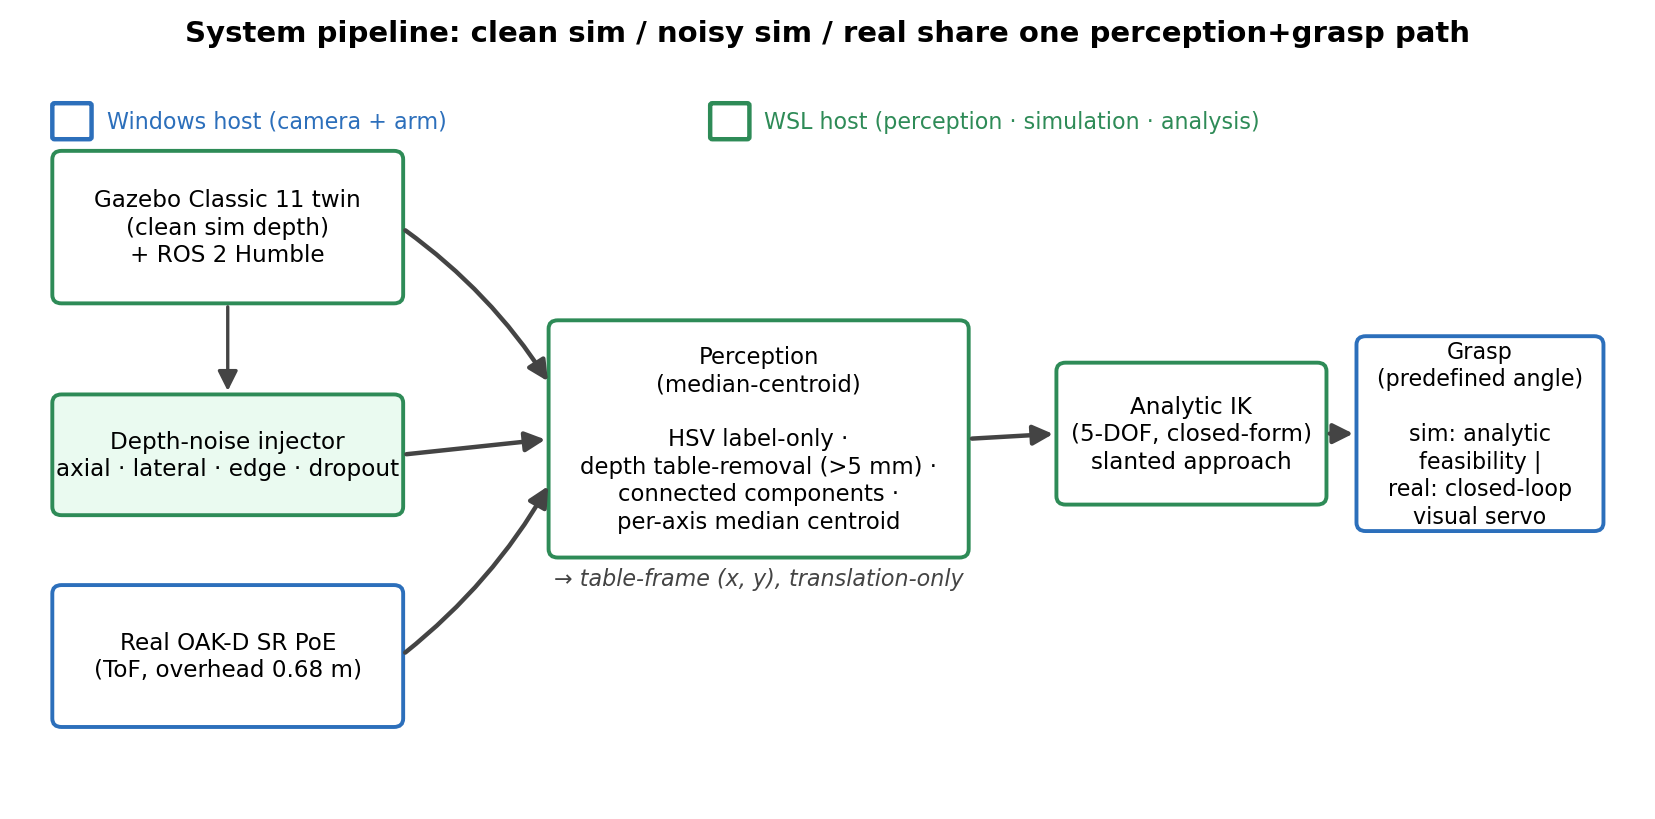
\includegraphics[width=0.92\textwidth]{system_pipeline.png}
\caption{System pipeline. Clean simulation, noise-injected simulation, and the real
OAK-D feed one shared perception$\rightarrow$IK$\rightarrow$grasp path, isolating depth
noise as the only variable. Box colour indicates the host: the camera and arm run on
Windows; perception, simulation, and analysis run under WSL.}
\label{fig:pipeline}
\end{figure*}

\subsection{Simulation and robot model}
The simulation uses Gazebo Classic~11 with ROS~2 Humble (Figure~\ref{fig:simscene}).
Control is provided through
\texttt{ros2\_control}, with a joint-trajectory controller for the arm and an effort/PID
controller for the gripper, integrated through a vendored build of
\texttt{gazebo\_ros2\_control} \cite{gazebo_ros2_control}. The arm is anchored to the
world by a fixed joint at $z=0.76$\,m so that it does not fall or drift, which keeps every
measured grasp error attributable to perception rather than to base motion.

The robot is a Hiwonder xArm~1S, a low-cost hobby arm. Its URDF was sourced from a
community model (GrabCAD; see Appendix~\ref{app:assets}) and modelled as a 5-DOF kinematic
chain followed by a parallel-jaw gripper: a base yaw joint, a planar three-revolute (3R)
sub-chain whose three pitch axes are parallel, and a wrist roll. The gripper is fixed
relative to the wrist, with the tool point offset $+0.09$\,m beyond the last
joint.\footnote{The proposal refers to the arm as 6-DoF; the implemented analytic
kinematics are 5-DOF, consistent with the URDF used.}

The camera is a Luxonis OAK-D SR PoE ToF unit \cite{luxonis_oakd}, mounted overhead and
pointing straight down at $0.68$\,m above the table. The same mount height is carried into
simulation, which removes eye-in-hand drift and isolates the depth axis as the variable of
interest. The stream is RGB-D at $640\times480$ with an approximately $60^\circ$ field of
view, accessed through DepthAI \cite{depthai_docs}; factory intrinsics are used
throughout, with no separate calibration run.

\begin{figure}[htbp]
\centering
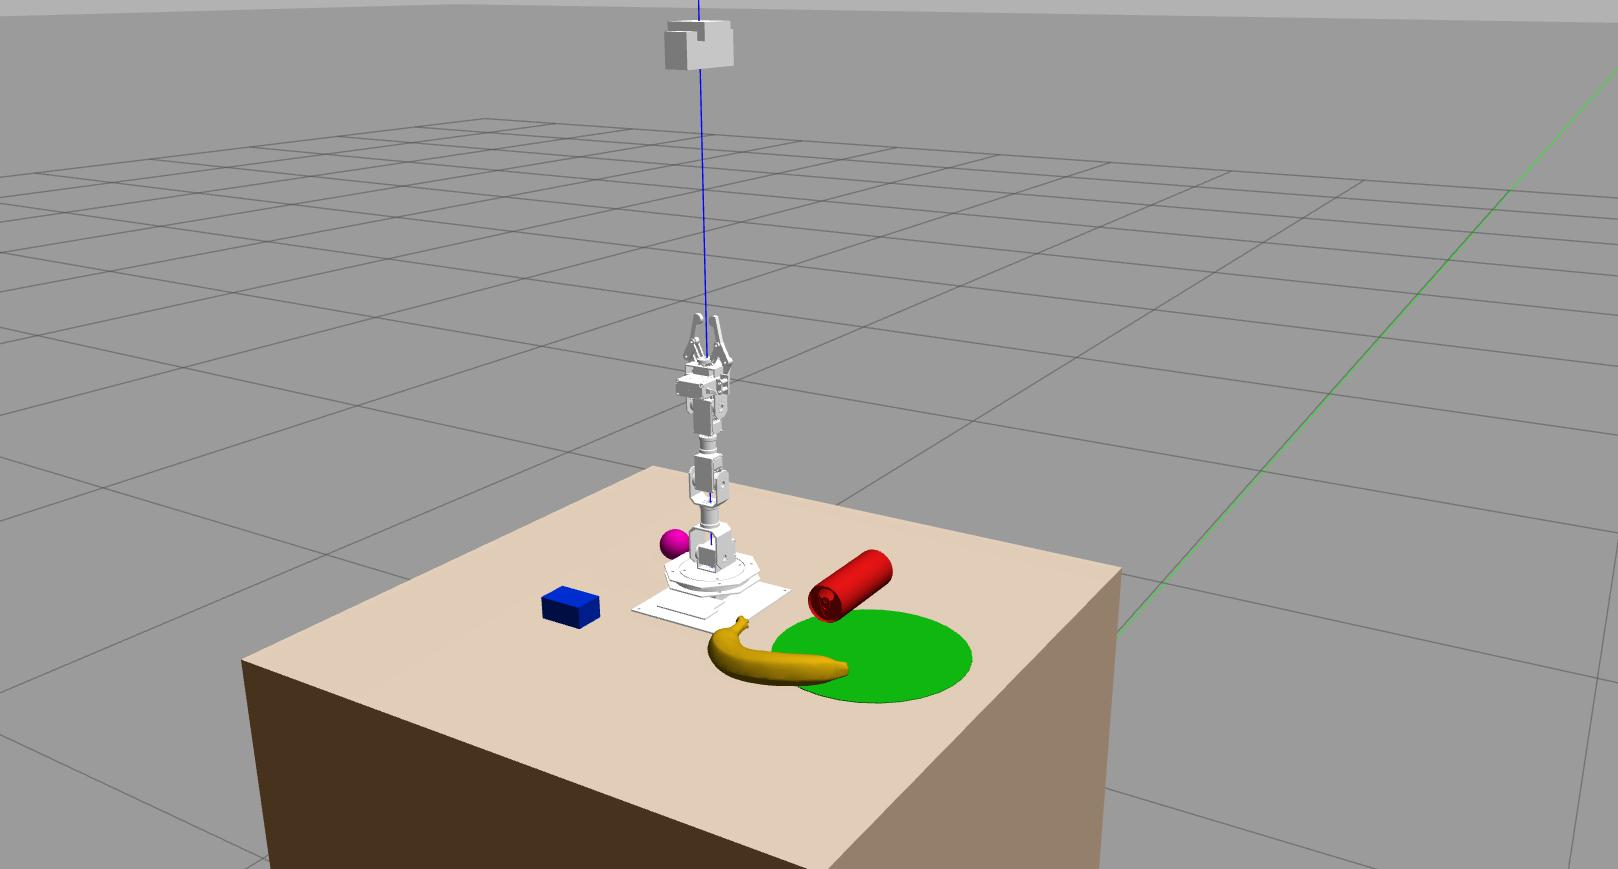
\includegraphics[width=\linewidth]{sim_scene.jpg}
\caption{The matched digital twin in Gazebo Classic: the simulated xArm~1S with its
parallel-jaw gripper over the tabletop, the four task objects (blue box, banana, red can,
and a sphere standing in for the golf ball), and the overhead OAK-D above. The same
geometry, mount height, and objects are used on the real system.}
\label{fig:simscene}
\end{figure}

\subsection{Analytic inverse kinematics}
Because the three pitch joints form a planar 3R arm, the arm position is solved in closed
form analytically in pure NumPy, following standard manipulator kinematics
\cite{craig2005robotics}, with an optional forward-kinematics cross-check. Avoiding a
numerical solver removes solver convergence as a confound, so any grasp error reflects
perception, not planning. A practical consequence of the table-mounted geometry is that a
purely vertical top-down grasp is infeasible at most reaches. A \texttt{feasible\_approach}
routine therefore searches for the steepest reachable slanted approach within the joint
limits; the achievable approach tilt degrades from near vertical close to the base to
roughly $70$--$80^\circ$ at far reach, which becomes relevant in the real manipulation
results.

\subsection{Real ToF noise characterisation}
The sensor was characterised with on-camera smoothing disabled so as to expose the raw
noise: the FPPN, optical, and wiggle corrections were left on, while the temporal and
median filters were turned off. Each capture aggregates 200 frames. Two protocols were
used. The planar protocol follows standard depth-camera characterisation practice
\cite{khoshelham2012accuracy}: a matte, fronto-parallel target is imaged at five distances
from $0.40$ to $0.80$\,m, and the per-pixel temporal standard deviation and bias are
estimated. The object protocol separates each object's body from a six-pixel edge ring,
motivated by the observation that ToF error concentrates at depth discontinuities as
flying or mixed pixels \cite{foix2011lockin,sarbolandi2015kinect}. Together these
protocols test how well the literature models \cite{nguyen2012modeling,khoshelham2012accuracy}
describe the OAK-D SR PoE in this setup.

\subsection{Depth-noise injection model}\label{sec:methods-inject}
The injector adds four literature noise terms, parameterised from the measured YAML, to
the clean simulated depth $z(u,v)$ before it reaches perception, which avoids modifying
Gazebo internals (Figure~\ref{fig:cleannoisy}). Writing the perturbed depth as $z'$, the
four terms are applied in sequence:
\begin{align}
\text{axial:}   &\quad z' = z + s\,\sigma_z(z)\,\eta, \label{eq:axial}\\
\text{lateral:} &\quad z'(u,v) = z\big(u+\Delta u,\,v+\Delta v\big), \label{eq:lateral}\\
\text{edge:}    &\quad z' = \alpha\,z_{\text{near}} + (1-\alpha)\,z_{\text{far}}, \label{eq:edge}\\
\text{dropout:} &\quad z' \to \varnothing. \label{eq:dropout}
\end{align}
In the axial term~\eqref{eq:axial}, $\eta\sim\mathcal{N}(0,1)$, $s$ is the axial-scale
multiplier, and the per-pixel standard deviation follows the Nguyen model
$\sigma_z(z)=a+b\,(z-z_0)^2$ \cite{nguyen2012modeling}. The lateral term~\eqref{eq:lateral}
resamples each output pixel from a neighbour offset by
$(\Delta u,\Delta v)\sim\mathcal{N}(0,\sigma_L^2)$, also from Nguyen, with the
incidence-angle term dropped because the overhead camera looks down the table normal
($\theta\approx0$) and $\sigma_L$ fixed to the literature value of $0.8$\,px. The edge
mixed-pixel term~\eqref{eq:edge} fires only at depth discontinuities, where
$\lvert\partial_u z\rvert+\lvert\partial_v z\rvert>\tau$, with probability $p_e$, replacing
the pixel by a convex mix ($\alpha\sim\mathcal{U}(0,1)$) of the nearest and farthest depth
in its $3\times3$ neighbourhood \cite{foix2011lockin,sarbolandi2015kinect}. The dropout
term~\eqref{eq:dropout} marks a pixel invalid with probability $p_d$, where $\varnothing$
denotes a dropped, no-return pixel \cite{sarbolandi2015kinect}.

The two noisy conditions differ only in their parameters. The measured model
\texttt{sim\_noisy\_oakd} sets $a=0.9$\,mm and $b=0$---a flat, range-independent axial
floor, consistent with the Phase-2 finding that the OAK-D's axial precision is
sub-millimetre and essentially flat with range---together with $\tau=2$\,cm, $p_e=0.70$ and
$p_d=0$, since no dropout was measured. The literature model \texttt{sim\_noisy\_nguyen}
instead uses Nguyen's Kinect coefficients $(a,b,z_0)=(0.0012,0.0019,0.4)$, $\tau=5$\,cm,
$p_e=0.30$ and $p_d=0.02$; both share $\sigma_L=0.8$\,px. To probe robustness, the axial
term is multiplied by an \texttt{axial\_scale} factor $s$ swept over $\{1,2,5,10,20\}$,
where $\times1$ is the measured level. The random number generator is seeded, with
independent streams for the continuous noise and the discrete masks, so that conditions are
directly comparable; the seeded ablation design is our own, in the spirit of controlled
randomisation studies \cite{tobin2017domain}. The third condition, \texttt{sim\_clean},
applies no injector.

\begin{figure}[htbp]
\centering
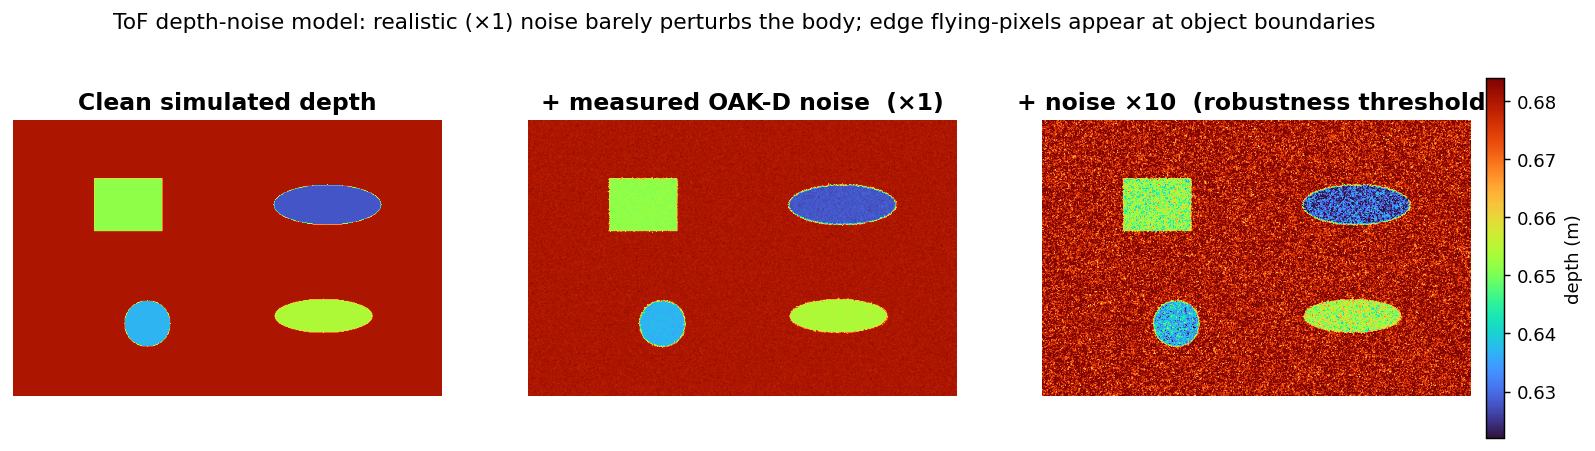
\includegraphics[width=\linewidth]{clean_vs_noisy_depth.png}
\caption{Simulated tabletop depth, clean versus the measured four-term ToF noise model
injected at $\times1$ and $\times10$. At the measured ($\times1$) level the object bodies
are barely perturbed and the added noise concentrates at edges; only at $\times10$ does
the field visibly degrade.}
\label{fig:cleannoisy}
\end{figure}

\subsection{Perception pipeline}\label{sec:methods-perc}
The perception module is classical and geometric by design. The RGB image is converted to
HSV and per-object colour masks are used only to label which blob is which; they never
contribute to geometry. The table is removed in depth: its plane depth is estimated as the
median of all valid depths, and any pixel at least $\delta=5$\,mm closer is marked as
object,
\begin{equation}
\begin{aligned}
z_{\text{table}} &= \operatorname{median}\{z(u,v)\},\\
\mathcal{O} &= \{(u,v): z(u,v)<z_{\text{table}}-\delta\}.
\end{aligned}
\label{eq:table}
\end{equation}
This step deliberately replaces RANSAC plane fitting \cite{rusu2008towards}, which is
unnecessary here because the support plane is known and fronto-parallel. Connected
components \cite{bradski2000opencv} then yield one blob per object. For each blob, the
valid pixels are back-projected with the pinhole intrinsics and reduced to a position by
the per-axis median of their coordinates,
\begin{equation}
\begin{aligned}
&X = (u-c_x)\,z/f_x,\quad Y = (v-c_y)\,z/f_y,\quad Z = z,\\
&\hat{\mathbf{c}} = \big(\operatorname{median}_i X_i,\ \operatorname{median}_i Y_i,\ \operatorname{median}_i Z_i\big),
\end{aligned}
\label{eq:median}
\end{equation}
giving a table-frame position (Figure~\ref{fig:perception}). The pose is translation-only
(3-DoF), with orientation set to identity.

The per-axis median is the crux of the entire study. It is an outlier-robust estimator
with a 50\% breakdown point \cite{huber1981robust}, and it is exactly what discards the
large edge flying-pixel population (between 53\% and 99\% of edge pixels, depending on
object) that constitutes the real noise. Finally, detections are matched to ground truth
by greedy nearest-neighbour assignment, a deliberate and documented simplification.

\begin{figure}[htbp]
\centering
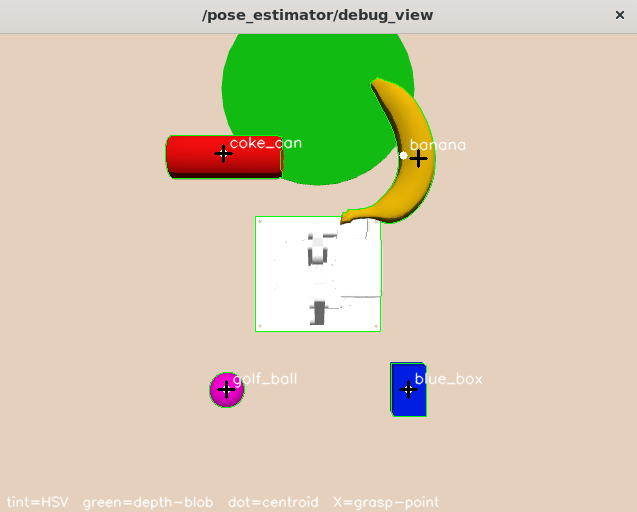
\includegraphics[width=\linewidth]{perception_debug.png}
\caption{Perception pipeline output (the \texttt{pose\_estimator} debug view): per-object
HSV colour labels (used only for identity, never for geometry), the depth blob (green), and
the per-object median centroid (dot) and predefined grasp point (X) for all four objects.
The position comes entirely from the depth blob; the colour tint never contributes to it.}
\label{fig:perception}
\end{figure}

\subsection{Grasp pipeline and feasibility metric}
Grasping uses a fixed, predefined per-object nominal grasp angle, identical in simulation
and on the real arm, which positions the predefined-grasp baseline discussed in the
grasping literature \cite{bohg2014grasp} rather than planning grasps online. Because
Gazebo Classic cannot reliably contact-grasp small or curved objects (finger collisions
pass through, and the object pose is bit-identical before and after closing the jaws), the
success metric is analytic rather than physical. A grasp is scored as feasible if and only
if the perceived object centre lies within the object's jaw capture tolerance of the true
centre, that is, if the open jaws would straddle the object. With per-object grasp width
$w$ and the measured gripper opening $W_{\text{jaw}}=55$\,mm, the jaw capture tolerance is
$\tau=(W_{\text{jaw}}-w)/2$, and feasibility is the planar test
\begin{equation}
\begin{aligned}
&\tau = (W_{\text{jaw}}-w)/2,\\
&e_{\text{cap}} = \lVert\hat{\mathbf{c}}_{xy}-\mathbf{c}^{*}_{xy}\rVert_2,\\
&\texttt{grasp\_feasible} = \mathbf{1}\!\left[\,e_{\text{cap}}\le\tau\,\right].
\end{aligned}
\label{eq:feasible}
\end{equation}
where $\hat{\mathbf{c}}_{xy}$ and $\mathbf{c}^{*}_{xy}$ are the perceived and true object
centres in the table plane. To avoid overclaiming, this metric is named
\texttt{grasp\_feasible} rather than pick success. For visualisation only,
a custom MIT plugin performs a contact-triggered fixed-joint attach following the
IFRA-Cranfield link-attacher pattern \cite{link_attacher}; it does not feed the measured
data.

\subsection{Real-world extrinsic calibration}\label{sec:methods-extrinsic}
For the real evaluation (Phase~4B), fiducials are detected on the OAK-D RGB camera rather
than on the ToF amplitude image, because the soft amplitude image yielded no usable
corners; the detections are then composed into the depth frame through the factory
RGB-to-ToF extrinsic. The camera-to-table transform is recovered from a printed
$7\times5$ ChArUco board (dictionary \texttt{DICT\_5X5\_100}, $100$\,mm squares) by direct
\texttt{solvePnP} \cite{garridojurado2014aruco,romeroramirez2018charuco}, with no hand-eye
calibration (Figure~\ref{fig:extrinsic}). The solution localised 20 of 24 corners at
$0.26$\,px reprojection error and placed the board at $0.683$\,m, in agreement to $1.4$\,mm
with the $0.684$\,m plane fitted to the depth image. Frame transforms are handled with the
ROS~2 transform library \cite{foote2013tf}.

\begin{figure}[htbp]
\centering
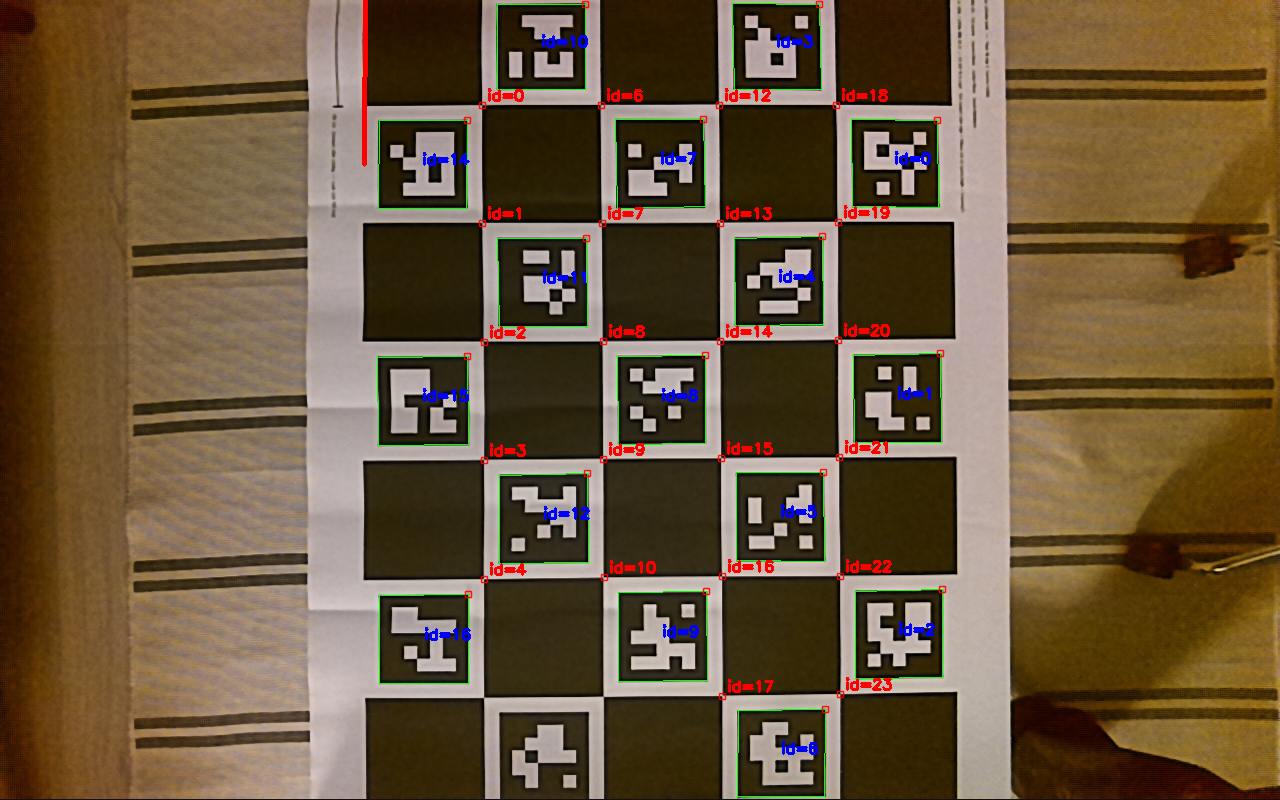
\includegraphics[width=\linewidth]{extrinsics_overlay.png}
\caption{The $7\times5$ ChArUco extrinsic board (\texttt{DICT\_5X5\_100}, $100$\,mm squares)
as imaged by the OAK-D's own RGB camera, with the OpenCV ArUco detection overlaid (green
marker boundaries, red ids). These marker and chessboard-corner correspondences feed the
direct \texttt{solvePnP} that recovers the camera-to-table extrinsic; the resulting board
height ($0.683$\,m) agrees with the depth-plane fit ($0.684$\,m) to $1.4$\,mm.}
\label{fig:extrinsic}
\end{figure}

\subsection{Real arm control and closed-loop visual servo}\label{sec:methods-servo}
The real arm is driven over USB-HID using a lightweight, ROS-free Python bridge. This
work, including the closed-loop executor below, is baseline and appendix material rather
than a results contribution; it exists so that the real grasp uses the same recipe as
simulation and the measured gap reflects execution rather than a perception confound. Two
real-to-model mismatches drive the design. First, the real gripper opens to $55$\,mm,
whereas the idealised URDF opened to $72$\,mm; the smaller real opening tightens the
tightest object's capture tolerance and is a disclosed source of sim-to-real difference.
Second, and more importantly, the real arm over-reaches the URDF kinematic model by
roughly 28\%,% TODO: confirm against the bench value -- the 0.777 scale implies 1/0.777 = 1.287, i.e. ~28.7% over-reach
 because the model link lengths do not match the physical arm. A global
similarity-scale table-to-arm transform of approximately $0.777$ (the reciprocal of the
over-reach factor, $1/1.287$) reduces this but leaves a
position-dependent residual of about $14$\,mm RMS over the workspace, which exceeds the
tightest object's tolerance and confines reliable open-loop grasping to a small patch of
the table.

The residual is an unidentifiable, position-dependent kinematic-model error, so no fixed
offset or low-parameter recalibration can remove it across the workspace. The adopted
solution closes the loop visually in a way that is independent of the broken kinematics
(Figure~\ref{fig:servo}). A single ArUco marker (dictionary \texttt{DICT\_4X4\_50}, id~4;
the object markers use ids 0--3) is taped flat on the gripper so the overhead camera sees
it. Before descending, the controller iterates in the table frame,
\begin{equation}
\mathbf{e} = \mathbf{p}_{\text{obj}} - \big(\mathbf{p}_{\text{marker}} + \mathbf{t}_{\text{tip}}\big),
\qquad \mathbf{target}\mathrel{+}= K\,\mathbf{e},
\end{equation}
with gain $K\approx0.6$, until $\lVert\mathbf{e}\rVert < 3$\,mm, after which it descends
and closes. Because the error is a difference of two points measured through the same
camera in the same frame, the incorrect forward kinematics and the global scale act as
common-mode bias and cancel; they only need to be good enough for the loop to converge.
Grasp accuracy then becomes camera-bound (on the order of $1$ to $4$\,mm) across the
workspace. A dense, camera-measured correction field, in the spirit of low-cost
reproducible-arm calibration work \cite{yang2019replab}, was prepared as a citable
open-loop fallback but was not needed, since the closed loop alone produced the result.

\begin{figure*}[t]
\centering
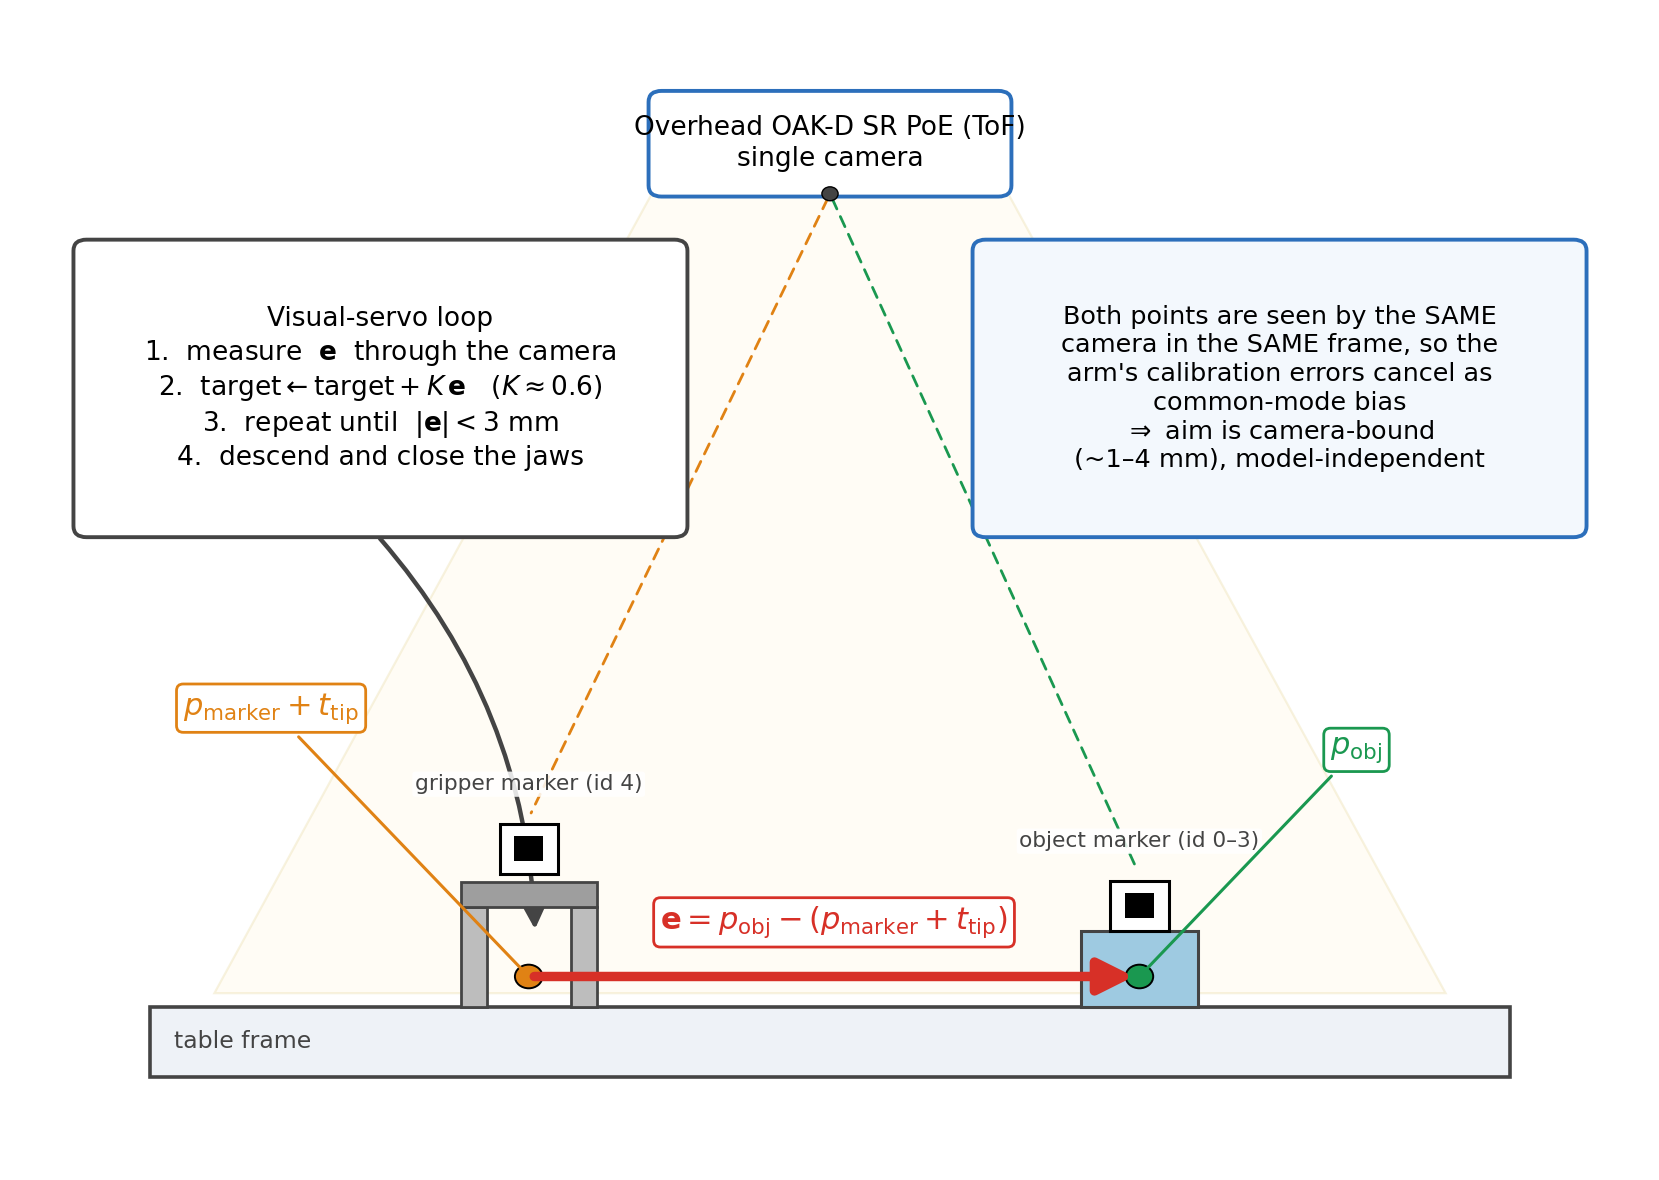
\includegraphics[width=0.86\textwidth]{servo_schematic.png}
\caption{Closed-loop visual-servo alignment (Phase~4C, baseline/Methods). The single
overhead camera measures the object point $\mathbf{p}_{\text{obj}}$ and the gripper-marker
point $\mathbf{p}_{\text{marker}}+\mathbf{t}_{\text{tip}}$ in the same table frame; the
inverse-kinematics target is nudged by $K\,\mathbf{e}$ until the in-frame error falls below
$3$\,mm. Because both points pass through the same camera, the incorrect forward kinematics
(a ${\sim}28\%$ over-reach) and the global $0.777$ scale cancel as common-mode bias and
aiming becomes camera-bound.}
\label{fig:servo}
\end{figure*}

% =====================================================================
